\documentclass[12pt,a4paper]{article}

% ─── Page Layout ───────────────────────────────────────────────────────────────
\usepackage[a4paper, margin=0.8in, headheight=14pt]{geometry}

% ─── Fonts (XeLaTeX) ───────────────────────────────────────────────────────────
\usepackage{fontspec}
\usepackage{unicode-math}
\setmainfont{TeX Gyre Pagella}
\setmonofont[Scale=0.88]{TeX Gyre Cursor}
\setmathfont{Latin Modern Math}

% ─── Packages ──────────────────────────────────────────────────────────────────
\usepackage{xcolor}
\usepackage{colortbl}
\usepackage{titlesec}
\usepackage{enumitem}
\usepackage{tabularx}
\usepackage{booktabs}
\usepackage{array}
\usepackage{amsmath}
\usepackage{tikz}
\usetikzlibrary{shapes.geometric, arrows.meta, positioning, calc, fit, decorations.pathreplacing, patterns}
\usepackage[american]{circuitikz}
\usepackage{tcolorbox}
\tcbuselibrary{skins, breakable}
\usepackage{hyperref}
\usepackage{fancyhdr}
\usepackage{graphicx}
\usepackage{microtype}
\hyphenpenalty=10000
\exhyphenpenalty=10000
\sloppy
\usepackage{caption}
\usepackage{setspace}
\usepackage{multirow}
\usepackage{tocloft}

% ─── Q&A helper ────────────────────────────────────────────────────────────────
\newcommand{\Q}[1]{\textbf{#1}\par\noindent\ignorespaces}

% ─── Colour Palette ────────────────────────────────────────────────────────────
\definecolor{myred}{RGB}{196,30,58}
\definecolor{mydark}{RGB}{30,30,50}
\definecolor{mygreen}{RGB}{14,120,80}
\definecolor{myteal}{RGB}{0,130,140}
\definecolor{myamber}{RGB}{180,100,0}
\definecolor{mypurple}{RGB}{100,30,160}
\definecolor{mygray}{RGB}{246,247,249}
\definecolor{mgframe}{RGB}{180,185,200}
\definecolor{watermark}{RGB}{145,150,170}
\definecolor{hdrred}{RGB}{250,232,235}
\definecolor{hdrgreen}{RGB}{220,244,233}
\definecolor{hdrteal}{RGB}{220,242,244}
\definecolor{hdramber}{RGB}{253,242,215}
\definecolor{hdrpurple}{RGB}{238,228,255}
\definecolor{hdrgray}{RGB}{238,240,245}
\definecolor{rowalt}{RGB}{250,251,253}

% ─── Section Formatting ────────────────────────────────────────────────────────
\titleformat{\section}{\large\bfseries\color{myred}}{\thesection.}{0.5em}{}[\vspace{1pt}{\color{myred}\rule{\linewidth}{0.8pt}}]
\titleformat{\subsection}{\normalsize\bfseries\color{myteal}}{\thesubsection}{0.5em}{}
\titlespacing*{\section}{0pt}{18pt}{7pt}
\titlespacing*{\subsection}{0pt}{11pt}{4pt}

% ─── Paragraph ─────────────────────────────────────────────────────────────────
\setlength{\parindent}{0pt}
\setlength{\parskip}{4pt}

% ─── TOC Styling ───────────────────────────────────────────────────────────────
\renewcommand{\cfttoctitlefont}{\large\bfseries\color{myred}}
\renewcommand{\cftaftertoctitle}{\par\noindent{\color{myred}\rule{\linewidth}{0.8pt}}}
\setlength{\cftbeforetoctitleskip}{0pt}
\setlength{\cftaftertoctitleskip}{6pt}
\renewcommand{\cftsecfont}{\normalsize\bfseries\color{mydark}}
\renewcommand{\cftsecpagefont}{\normalsize\bfseries\color{mydark}}
\renewcommand{\cftsecleader}{\cftdotfill{\cftdotsep}}
\setlength{\cftbeforesecskip}{7pt}
\renewcommand{\cftsubsecfont}{\small\color{mydark}}
\renewcommand{\cftsubsecpagefont}{\small\color{mydark}}
\setlength{\cftbeforesubsecskip}{3pt}
\setlength{\cftsubsecindent}{1.4em}

% ─── Table helpers ─────────────────────────────────────────────────────────────
\renewcommand{\arraystretch}{1.45}
\setlength{\tabcolsep}{6pt}
\arrayrulecolor{mydark}
\newcolumntype{B}[1]{>{\small\bfseries\raggedright\arraybackslash}m{#1}}
\newcolumntype{Y}{>{\small\raggedright\arraybackslash}X}
\renewcommand{\tabularxcolumn}[1]{m{#1}}

% ─── Header / Footer ───────────────────────────────────────────────────────────
\pagestyle{fancy}
\fancyhf{}
\fancyhead[L]{\small\color{myred}\textbf{PE-EC802C}\;\color{mydark}--- VLSI Design Automation}
\fancyhead[R]{\small\color{myteal}\textbf{Module 5 Notes}}
\fancyfoot[C]{\small\color{mydark}\thepage}
\fancyfoot[R]{\small\color{watermark}\textit{\copyright\ Biraj Sarkar}}
\renewcommand{\headrulewidth}{0.5pt}
\renewcommand{\footrulewidth}{0.3pt}

% ─── Hyperref ──────────────────────────────────────────────────────────────────
\hypersetup{colorlinks=true, linkcolor=myteal, urlcolor=myteal,
  pdfauthor={Biraj Sarkar}, pdftitle={PE-EC802C --- Module 5 Notes}}

% ─── tcolorbox styles ──────────────────────────────────────────────────────────
\tcbset{
  tikzbox/.style={colback=mygray, colframe=mgframe, boxrule=0.6pt, arc=4pt,
    left=8pt, right=8pt, top=6pt, bottom=6pt,
    colbacktitle=mgframe, coltitle=mydark, fonttitle=\small\bfseries},
  defbox/.style={colback=hdrgreen, colframe=mygreen, boxrule=0.8pt, arc=4pt,
    left=9pt, right=9pt, top=6pt, bottom=6pt,
    colbacktitle=mygreen, coltitle=white, fonttitle=\small\bfseries},
  formulabox/.style={colback=hdrteal, colframe=myteal, boxrule=0.8pt, arc=4pt,
    left=9pt, right=9pt, top=7pt, bottom=7pt,
    colbacktitle=myteal, coltitle=white, fonttitle=\small\bfseries},
  examplebox/.style={colback=hdramber, colframe=myamber, boxrule=0.8pt, arc=4pt,
    left=9pt, right=9pt, top=6pt, bottom=6pt,
    colbacktitle=myamber, coltitle=white, fonttitle=\small\bfseries},
  masonbox/.style={colback=hdrpurple, colframe=mypurple, boxrule=0.8pt, arc=4pt,
    left=9pt, right=9pt, top=6pt, bottom=6pt,
    colbacktitle=mypurple, coltitle=white, fonttitle=\small\bfseries},
  exambox/.style={colback=hdrpurple, colframe=mypurple, boxrule=1pt, arc=5pt,
    left=10pt, right=10pt, top=8pt, bottom=8pt,
    colbacktitle=mypurple, coltitle=white, fonttitle=\bfseries,
    breakable, title after break={\textbf{Frequently Asked / Viva Questions (contd.)}}}
}
\tcbset{breakable}

% ─── TikZ styles ───────────────────────────────────────────────────────────────
\tikzset{
  block/.style={rectangle, draw=myteal, fill=hdrteal,
    text width=2.4cm, align=center, minimum height=0.95cm,
    font=\small, rounded corners=3pt, line width=0.7pt},
  redblock/.style={rectangle, draw=myred, fill=hdrred,
    text width=2.4cm, align=center, minimum height=0.95cm,
    font=\small, rounded corners=3pt, line width=0.7pt},
  sumjunc/.style={circle, draw=myamber, fill=hdramber,
    minimum size=0.62cm, font=\small, line width=0.8pt},
  arrow/.style={-Stealth, thick, color=mydark},
  line/.style={thick, color=mydark}
}

% ═══════════════════════════════════════════════════════════════════════════════
\begin{document}
% ═══════════════════════════════════════════════════════════════════════════════

\begin{center}
  {\LARGE\bfseries\color{myred} PE-EC802C --- VLSI Design Automation}\\[5pt]
  {\normalsize\color{mydark} Semester VIII \quad$\bullet$\quad 3L:0T:0P \quad$\bullet$\quad 3 Credits}\\[3pt]
  {\normalsize\color{myteal}\textbf{Module 5: High-Level Synthesis}}\\[3pt]
  {\small\color{mydark} CGEC \;$|$\; B.Tech ECE (2023--27) \;$|$\; \textit{Biraj Sarkar}}
\end{center}
\vspace{2pt}
\noindent{\color{myred}\rule{\linewidth}{1.5pt}}
\vspace{2pt}

\hypersetup{linkcolor=mydark}
\tableofcontents
\hypersetup{linkcolor=myteal}
\newpage

% ===============================================================================
\section{High-Level Synthesis (HLS) Core Concepts}
% ===============================================================================

\begin{tcolorbox}[defbox, title={High-Level Synthesis}]
  \textbf{High-Level Synthesis (HLS)} is the automated design process that translates an algorithmic description of behavior (written in C, C++, SystemC) into a Register Transfer Level (RTL) description (written in Verilog or VHDL) implementing a digital circuit controller and datapath.
\end{tcolorbox}

\subsection{Core Compilation Steps}
The HLS process consists of three main subproblems that are closely coupled:
\begin{enumerate}[leftmargin=*, itemsep=2pt]
  \item \textbf{Scheduling:} Assigning each operation in the algorithm to a specific execution control step (clock cycle) while respecting data dependencies and resource bounds.
  \item \textbf{Allocation:} Selecting the types and quantities of hardware resources (e.g. 2 adders, 1 multiplier) to implement the operations, registers, and buses.
  \item \textbf{Binding (Assignment):} Mapping each operation to a specific allocated functional unit (e.g., mapping multiplication $v_3$ to multiplier $M_1$) and mapping variables to specific registers.
\end{enumerate}

\subsection{Hardware \& Architecture Models in HLS}
HLS tools map behavioral code onto specific structural hardware templates. The primary target model is the \textbf{Controller-Datapath Model} (Finite State Machine with Datapath, FSMD):
\begin{itemize}[leftmargin=*, itemsep=3pt]
  \item \textbf{Datapath:} Contains functional units (ALUs, multipliers, adders) for arithmetic execution, registers/memories for data storage, and multiplexers/buses for routing data.
  \item \textbf{Controller:} An FSM that generates control signals (write enables, mux select lines) for each control step and reads status signals (flags, comparisons) from the datapath.
\end{itemize}
Microarchitectural models of functional units include:
\begin{itemize}[leftmargin=*, itemsep=2pt]
  \item \textbf{Combinational Units:} Complete execution within a single clock cycle (e.g. basic adders).
  \item \textbf{Multi-cycle Units:} Take $d \ge 2$ clock cycles to execute. No new inputs can be accepted until execution finishes (e.g. non-pipelined dividers).
  \item \textbf{Pipelined Units:} Take $d \ge 2$ clock cycles but can accept new inputs every $II$ (Initiation Interval) cycles (e.g. pipelined multipliers).
\end{itemize}

\subsection{Internal Representations}
\begin{itemize}[leftmargin=*, itemsep=2pt]
  \item \textbf{Data Flow Graph (DFG):} A directed acyclic graph where vertices represent arithmetic operations ($+, -, \times$) and directed edges represent data dependencies (values passed from one operation to another).
  \item \textbf{Control Data Flow Graph (CDFG):} An extension of the DFG that includes control flow structures (loops, conditional branches `if-else`, jumps). Vertices represent basic blocks of operations, and edges represent control decisions.
\end{itemize}

\begin{tcolorbox}[tikzbox, title={Data Flow Graph for $y = (a + b) \cdot (c - d)$}]
\centering
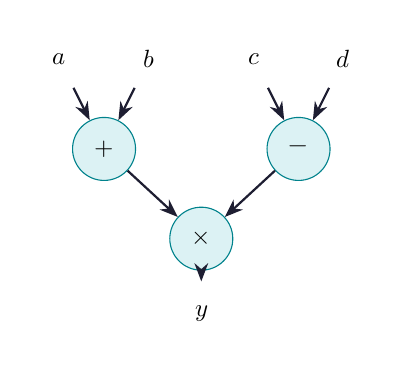
\begin{tikzpicture}[scale=0.95, every node/.style={circle, draw=myteal, fill=hdrteal, minimum size=0.8cm, font=\small}]
  % Inputs
  \node[draw=none, fill=none] (a) at (0,2.4) {$a$};
  \node[draw=none, fill=none] (b) at (1.2,2.4) {$b$};
  \node[draw=none, fill=none] (c) at (2.6,2.4) {$c$};
  \node[draw=none, fill=none] (d) at (3.8,2.4) {$d$};

  % Operators
  \node (add) at (0.6,1.2) {$+$};
  \node (sub) at (3.2,1.2) {$-$};
  \node (mul) at (1.9,0) {$\times$};
  
  % Output
  \node[draw=none, fill=none] (y) at (1.9,-1.0) {$y$};

  % Edges
  \draw[arrow] (a) -- (add);
  \draw[arrow] (b) -- (add);
  \draw[arrow] (c) -- (sub);
  \draw[arrow] (d) -- (sub);
  \draw[arrow] (add) -- (mul);
  \draw[arrow] (sub) -- (mul);
  \draw[arrow] (mul) -- (y);
\end{tikzpicture}
\end{tcolorbox}

% ===============================================================================
\section{Scheduling Algorithms}
% ===============================================================================

Scheduling decides the overall trade-off between latency (clock cycles) and circuit area (number of functional units).

\subsection{1. ASAP Scheduling (As-Soon-As-Possible)}
ASAP is an unconstrained scheduling algorithm that schedules each operation to the earliest possible control step as soon as all its predecessor inputs are available.
\begin{itemize}[leftmargin=*, itemsep=2pt]
  \item \textbf{Formula:} Start time $t_i = 1$ if node $i$ has no predecessors; otherwise:
        \begin{equation}
          t_i = \max_{j \in \text{Pred}(i)} (t_j + d_j)
        \end{equation}
        where $d_j$ is the execution delay of predecessor node $j$ (usually 1 cycle).
\end{itemize}

\subsection{2. ALAP Scheduling (As-Late-As-Possible)}
ALAP schedules each operation to the latest possible control step without violating a predefined maximum latency constraint $L$ cycles.
\begin{itemize}[leftmargin=*, itemsep=2pt]
  \item \textbf{Formula:} Start time $t_i = L$ if node $i$ has no successors; otherwise:
        \begin{equation}
          t_i = \min_{j \in \text{Succ}(i)} (t_j) - d_i
        \end{equation}
\end{itemize}

\begin{tcolorbox}[tikzbox, title={ASAP vs. ALAP Scheduling Timelines (Latency constraint $L = 3$)}]
\centering
\begin{minipage}{0.48\linewidth}
\centering
\textbf{ASAP Scheduling:}\par\noindent
\vspace{6pt}
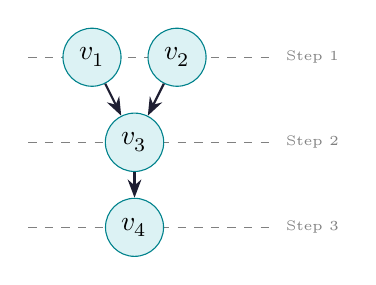
\begin{tikzpicture}[scale=0.9]
  % Grid steps
  \draw[dashed, gray] (-0.5,0) -- (3.0,0) node[right, font=\tiny] {Step 3};
  \draw[dashed, gray] (-0.5,1.2) -- (3.0,1.2) node[right, font=\tiny] {Step 2};
  \draw[dashed, gray] (-0.5,2.4) -- (3.0,2.4) node[right, font=\tiny] {Step 1};

  % Nodes
  \node[circle, draw=myteal, fill=hdrteal, minimum size=0.6cm] (n1) at (0.4,2.4) {$v_1$};
  \node[circle, draw=myteal, fill=hdrteal, minimum size=0.6cm] (n2) at (1.6,2.4) {$v_2$};
  \node[circle, draw=myteal, fill=hdrteal, minimum size=0.6cm] (n3) at (1.0,1.2) {$v_3$};
  \node[circle, draw=myteal, fill=hdrteal, minimum size=0.6cm] (n4) at (1.0,0) {$v_4$};

  % Connections
  \draw[arrow] (n1) -- (n3);
  \draw[arrow] (n2) -- (n3);
  \draw[arrow] (n3) -- (n4);
\end{tikzpicture}
\end{minipage}\hfill
\begin{minipage}{0.48\linewidth}
\centering
\textbf{ALAP Scheduling:}\par\noindent
\vspace{6pt}
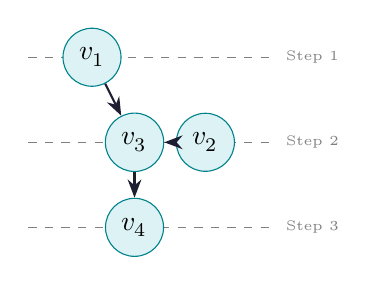
\begin{tikzpicture}[scale=0.9]
  % Grid steps
  \draw[dashed, gray] (-0.5,0) -- (3.0,0) node[right, font=\tiny] {Step 3};
  \draw[dashed, gray] (-0.5,1.2) -- (3.0,1.2) node[right, font=\tiny] {Step 2};
  \draw[dashed, gray] (-0.5,2.4) -- (3.0,2.4) node[right, font=\tiny] {Step 1};

  % Nodes (v2 delayed to step 2)
  \node[circle, draw=myteal, fill=hdrteal, minimum size=0.6cm] (n1) at (0.4,2.4) {$v_1$};
  \node[circle, draw=myteal, fill=hdrteal, minimum size=0.6cm] (n2) at (2.0,1.2) {$v_2$};
  \node[circle, draw=myteal, fill=hdrteal, minimum size=0.6cm] (n3) at (1.0,1.2) {$v_3$};
  \node[circle, draw=myteal, fill=hdrteal, minimum size=0.6cm] (n4) at (1.0,0) {$v_4$};

  % Connections
  \draw[arrow] (n1) -- (n3);
  \draw[arrow] (n2) -- (n3);
  \draw[arrow] (n3) -- (n4);
\end{tikzpicture}
\end{minipage}
\tcblower
The range between ASAP and ALAP start times ($[t_{ASAP}, t_{ALAP}]$) represents the \textbf{slack} or mobility of an operation. If $t_{ASAP} = t_{ALAP}$, the operation lies on the critical path and has zero mobility.
\end{tcolorbox}

\subsection{3. List Scheduling}
A resource-constrained heuristic scheduling algorithm. It resolves scheduling step-by-step using a priority queue:
\begin{enumerate}[leftmargin=*, itemsep=2pt]
  \item Compute priority metrics for all operations (e.g. mobility, path length to sink).
  \item For each control step $t = 1, 2, \dots$:
    \begin{itemize}[leftmargin=*, label=$\bullet$, itemsep=1.5pt]
      \item Identify the \textbf{ready list} of operations whose predecessors have completed execution.
      \item Sort the ready list in descending order of priority.
      \item Schedule the highest priority operations to the available functional units.
      \item Defer the remaining ready operations to the next control step.
    \end{itemize}
\end{enumerate}

\subsection{4. Force-Directed Scheduling (FDS)}
FDS is a latency-constrained algorithm that minimizes resource costs by distributing operations of the same type uniformly across all control steps.
\begin{itemize}[leftmargin=*, itemsep=2pt]
  \item \textbf{Probability:} The probability that operation $i$ is scheduled in control step $t$ is $p_i(t) = \frac{1}{\mu_i + 1}$ for $t \in [t_{ASAP}, t_{ALAP}]$, where $\mu_i$ is mobility.
  \item \textbf{Distribution Graph (DG):} The sum of probabilities of all operations of type $op$ at step $t$: $DG(t) = \sum_{i} p_i(t)$.
  \item \textbf{Forces:} Calculates the attractive and repulsive forces between operations and control steps to place operations in slots with low distribution density, smoothing resource utilization.
\end{itemize}

% ===============================================================================
\section{Hardware Binding \& Transformations}
% ===============================================================================

Binding maps variables to registers and operations to functional units.

\subsection{The Assignment (Binding) Problem Formulation}
The binding (assignment) problem maps operations to functional units (resource allocation constraint) and variables to registers (storage allocation constraint). It can be formulated in different mathematical ways:
\begin{itemize}[leftmargin=*, itemsep=4pt]
  \item \textbf{Graph Coloring / Max-Clique Formulation:}
        \begin{itemize}[leftmargin=*, label=$\bullet$, itemsep=2pt]
          \item Create a \textbf{Compatibility Graph} where vertices represent operations (or variables) and edges connect vertices that can share the same resource (i.e., operations scheduled in different control steps, or variables with non-overlapping lifetimes).
          \item Finding a minimum clique partition in the compatibility graph (or coloring the conflict/clash graph) yields the optimal number of resources.
        \end{itemize}
  \item \textbf{Bipartite Matching Formulation:}
        \begin{itemize}[leftmargin=*, label=$\bullet$, itemsep=2pt]
          \item Maps operations to compatible functional units as a bipartite matching problem to minimize total steering logic (multiplexers and buses).
        \end{itemize}
  \item \textbf{Integer Linear Programming (ILP) Formulation:}
        \begin{itemize}[leftmargin=*, label=$\bullet$, itemsep=2pt]
          \item Let $x_{v,f} = 1$ if operation $v$ is bound to functional unit $f$.
          \item Subject to: $\sum_{f} x_{v,f} = 1$ (every operation is bound to exactly one unit).
          \item Subject to: $x_{v_1,f} + x_{v_2,f} \le 1$ for any two operations $v_1, v_2$ scheduled in the same control step (resource sharing constraint).
        \end{itemize}
\end{itemize}

\subsection{1. Register Binding (Left-Edge Algorithm)}
Variables that do not have overlapping lifetimes can share the same hardware register.
\begin{itemize}[leftmargin=*, itemsep=2pt]
  \item \textbf{Lifetime Interval:} The span between the control step where the variable is generated and the control step where it is last read.
  \item Left-Edge algorithm binds overlapping lifetime intervals to a minimum set of registers, identical to channel routing track allocation.
\end{itemize}

\subsection{2. High-Level Optimisation Transformations}
Before scheduling, HLS tools optimize the algorithmic code structure to improve performance:
\begin{itemize}[leftmargin=*, itemsep=2pt]
  \item \textbf{Loop Unrolling:} Duplicates loop bodies to expose parallel operations, reducing execution latency at the cost of larger circuit area.
  \item \textbf{Loop Pipelining:} Overlaps the execution of subsequent loop iterations in a pipelined fashion, starting iteration $k+1$ before iteration $k$ finishes.
  \item \textbf{Tree Height Reduction:} Reorganizes expression evaluations using algebraic properties (associativity, commutativity) to balance parsing trees and reduce critical path delay.
\end{itemize}

\newpage

% ═══════════════════════════════════════════════════════════════════════════════
% QUICK REVISION PAGE
% ═══════════════════════════════════════════════════════════════════════════════
\begin{center}
  {\large\bfseries\color{myred} Quick Revision — Module 5}\\[3pt]
  {\small\color{mydark} High-Level Synthesis $|$ PE-EC802C}
\end{center}
\noindent{\color{myred}\rule{\linewidth}{1.2pt}}
\vspace{8pt}

\begin{tcolorbox}[formulabox, title={\textbf{Key Formulas and Metrics at a Glance}}]
\renewcommand{\arraystretch}{1.35}
\begin{tabularx}{\linewidth}{B{5.0cm} X}
  Operation Mobility & $\mu_i = t_{i,\text{ALAP}} - t_{i,\text{ASAP}} \quad (\text{slack or scheduling freedom})$ \\[4pt]
  ASAP Scheduling & $t_{i,\text{ASAP}} = \max_{j \in \text{Pred}(i)} \left( t_{j,\text{ASAP}} + d_j \right)$ \\[4pt]
  ALAP Scheduling & $t_{i,\text{ALAP}} = \min_{k \in \text{Succ}(i)} \left( t_{k,\text{ALAP}} \right) - d_i$ \\[4pt]
  FDS Operation Prob. & $p_i(t) = \dfrac{1}{\mu_i + 1} \quad \text{for } t \in [t_{i,\text{ASAP}}, t_{i,\text{ALAP}}]$
\end{tabularx}
\end{tcolorbox}

\vspace{6pt}

\begin{tcolorbox}[defbox, title={\textbf{One-Line Definitions}}]
\begin{itemize}[leftmargin=*, itemsep=3pt, topsep=0pt]
  \item \textbf{Datapath:} The hardware block containing ALUs, multipliers, registers, and multiplexers that process data.
  \item \textbf{Controller:} The FSM block that generates control signals to coordinate datapath operations.
  \item \textbf{ASAP:} An unconstrained scheduling method that schedules operations at their earliest possible cycle.
  \item \textbf{ALAP:} A latency-constrained scheduling method that schedules operations at their latest possible cycle.
  \item \textbf{FDS:} An algorithm that minimizes functional units by distributing operations evenly across cycles.
  \item \textbf{Allocation:} Specifying the total hardware resources available to implement the design.
  \item \textbf{Binding:} Assigning logical operations and variables to specific physical functional units and registers.
  \item \textbf{Loop Unrolling:} A compiler optimization that replicates loop bodies to increase parallel operation opportunities.
  \item \textbf{Tree Height Reduction:} Reducing the depth of an expression tree using algebraic laws to speed up evaluation.
\end{itemize}
\end{tcolorbox}

\vspace{6pt}

\begin{tcolorbox}[exambox, title={\textbf{Frequently Asked / Viva Questions}}]
\begin{enumerate}[leftmargin=*, topsep=0pt, label=\textbf{Q\arabic*.}, itemsep=6pt]
  \item \Q{What are the three main subproblems in High-Level Synthesis?}
        (1) Scheduling (assigning operations to clock cycles), (2) Allocation (determining the type and number of hardware resources), and (3) Binding (assigning operations and variables to specific hardware units).
        
  \item \Q{Explain how register allocation can be modeled as a Graph Coloring problem.}
        A variable lifetime conflict graph is constructed where vertices represent variables, and an edge connects two vertices if their lifetimes overlap. Coloring this graph such that no two adjacent vertices share the same color maps directly to register binding. The minimum number of colors corresponds to the minimum number of registers needed.
        
  \item \Q{What is mobility in High-Level Synthesis scheduling, and why is it important?}
        Mobility is the difference between an operation's ALAP and ASAP start times. It represents the scheduling freedom (slack) of the operation. Zero mobility means the operation lies on the critical path, while high mobility allows the scheduler to shift the operation to resolve resource bottlenecks.
        
  \item \Q{Explain the concept of Loop Pipelining in HLS.}
        Loop pipelining allows successive loop iterations to execute concurrently without waiting for the previous iteration to finish. The rate at which new iterations start is called the Initiation Interval (II). Pipelining increases throughput dramatically.
        
  \item \Q{What is the difference between Resource-Constrained and Latency-Constrained scheduling?}
        Resource-constrained scheduling minimizes latency given a fixed limit on hardware units (e.g. List Scheduling). Latency-constrained scheduling minimizes the hardware unit cost given a fixed maximum execution time (e.g. ALAP, FDS).
        
  \item \Q{How does Tree Height Reduction reduce critical path delay?}
        Consider evaluating $a+b+c+d$. Sequential evaluation $((a+b)+c)+d$ has a depth of 3 adder stages. Using associativity, we can compute $(a+b)+(c+d)$ in a tree format with a depth of only 2 stages, reducing execution delay.
        
  \item \Q{What is functional unit binding, and what is its goal?}
        Functional unit binding assigns scheduled operations (e.g. additions) to specific physical components (e.g., Adder 1). The goal is to maximize sharing, which minimizes the total area of functional units, multiplexers, and interconnect buses.
        
  \item \Q{Explain how the Left-Edge algorithm is used in Register Binding.}
        It sorts variables by the start of their lifetimes. It then assigns non-overlapping variable lifetimes to the same register track sequentially, maximizing register sharing and minimizing the total register count.
        
  \item \Q{What is the role of the FSM controller in the generated RTL netlist?}
        The Finite State Machine (FSM) controller generates the control signals (e.g. multiplexer select lines, register write enables) at each clock cycle, coordinating the datapath to execute operations in the scheduled order.
        
  \item \Q{Why is high-level synthesis preferred over writing manual RTL?}
        HLS allows designing at a higher level of abstraction (C/C++), which speeds up development, makes verification easier, and allows designers to quickly explore different trade-offs between area and speed by changing scheduling constraints.
\end{enumerate}
\end{tcolorbox}

\vspace{6pt}

\begin{tcolorbox}[tikzbox, title={\textbf{Comparison Snapshot}}]
\textbf{ASAP vs. ALAP Scheduling:}\par\vspace{6pt}\noindent
{\renewcommand{\arraystretch}{1.35}%
\begin{tabularx}{\linewidth}{|B{3.2cm}|Y|Y|}
\hline
\textbf{Feature} & \textbf{ASAP Scheduling} & \textbf{ALAP Scheduling} \\
\hline
Constraints & Unconstrained (assumes infinite resources). & Latency-constrained (limited to $L$ cycles). \\
\hline
Goal & Finds the minimum possible latency boundary. & Finds the latest start times to delay operations. \\
\hline
Search Order & Topological search starting from source nodes. & Reverse topological search starting from sink nodes. \\
\hline
\end{tabularx}}

\vspace{12pt}
\textbf{DFG vs. CDFG:}\par\vspace{6pt}\noindent
{\renewcommand{\arraystretch}{1.35}%
\begin{tabularx}{\linewidth}{|B{3.2cm}|Y|Y|}
\hline
\textbf{Feature} & \textbf{Data Flow Graph (DFG)} & \textbf{Control Data Flow Graph (CDFG)} \\
\hline
Information & Models only data dependencies and arithmetic operations. & Models both data dependencies and control decisions. \\
\hline
Branches/Loops & Cannot represent loops or conditional branches. & Explicitly models loop jumps and conditional branches. \\
\hline
Use Case & Used for basic scheduling and binding. & Used for full behavioral synthesis of systems. \\
\hline
\end{tabularx}}
\end{tcolorbox}

\end{document}
